% Options for packages loaded elsewhere
\PassOptionsToPackage{unicode}{hyperref}
\PassOptionsToPackage{hyphens}{url}
%
\documentclass[
]{article}
\usepackage{lmodern}
\usepackage{amssymb,amsmath}
\usepackage{ifxetex,ifluatex}
\ifnum 0\ifxetex 1\fi\ifluatex 1\fi=0 % if pdftex
  \usepackage[T1]{fontenc}
  \usepackage[utf8]{inputenc}
  \usepackage{textcomp} % provide euro and other symbols
\else % if luatex or xetex
  \usepackage{unicode-math}
  \defaultfontfeatures{Scale=MatchLowercase}
  \defaultfontfeatures[\rmfamily]{Ligatures=TeX,Scale=1}
\fi
% Use upquote if available, for straight quotes in verbatim environments
\IfFileExists{upquote.sty}{\usepackage{upquote}}{}
\IfFileExists{microtype.sty}{% use microtype if available
  \usepackage[]{microtype}
  \UseMicrotypeSet[protrusion]{basicmath} % disable protrusion for tt fonts
}{}
\makeatletter
\@ifundefined{KOMAClassName}{% if non-KOMA class
  \IfFileExists{parskip.sty}{%
    \usepackage{parskip}
  }{% else
    \setlength{\parindent}{0pt}
    \setlength{\parskip}{6pt plus 2pt minus 1pt}}
}{% if KOMA class
  \KOMAoptions{parskip=half}}
\makeatother
\usepackage{xcolor}
\IfFileExists{xurl.sty}{\usepackage{xurl}}{} % add URL line breaks if available
\IfFileExists{bookmark.sty}{\usepackage{bookmark}}{\usepackage{hyperref}}
\hypersetup{
  pdftitle={Validation},
  pdfauthor={Tina Lasisi},
  hidelinks,
  pdfcreator={LaTeX via pandoc}}
\urlstyle{same} % disable monospaced font for URLs
\usepackage[margin=1in]{geometry}
\usepackage{longtable,booktabs}
% Correct order of tables after \paragraph or \subparagraph
\usepackage{etoolbox}
\makeatletter
\patchcmd\longtable{\par}{\if@noskipsec\mbox{}\fi\par}{}{}
\makeatother
% Allow footnotes in longtable head/foot
\IfFileExists{footnotehyper.sty}{\usepackage{footnotehyper}}{\usepackage{footnote}}
\makesavenoteenv{longtable}
\usepackage{graphicx,grffile}
\makeatletter
\def\maxwidth{\ifdim\Gin@nat@width>\linewidth\linewidth\else\Gin@nat@width\fi}
\def\maxheight{\ifdim\Gin@nat@height>\textheight\textheight\else\Gin@nat@height\fi}
\makeatother
% Scale images if necessary, so that they will not overflow the page
% margins by default, and it is still possible to overwrite the defaults
% using explicit options in \includegraphics[width, height, ...]{}
\setkeys{Gin}{width=\maxwidth,height=\maxheight,keepaspectratio}
% Set default figure placement to htbp
\makeatletter
\def\fps@figure{htbp}
\makeatother
\setlength{\emergencystretch}{3em} % prevent overfull lines
\providecommand{\tightlist}{%
  \setlength{\itemsep}{0pt}\setlength{\parskip}{0pt}}
\setcounter{secnumdepth}{-\maxdimen} % remove section numbering

\title{Validation}
\author{Tina Lasisi}
\date{2020-12-20 16:01:08}

\begin{document}
\maketitle

\hypertarget{curvature}{%
\section{Curvature}\label{curvature}}

Here, we will evaluate the accuracy of \emph{fibermorph} in estimating
the length and curvature of hair using simulated data. See simulation
script
\href{https://github.com/tinalasisi/2020_HairPheno_manuscript/blob/main/code/simhair.R}{here}.

The simulated data can be found
\href{https://github.com/tinalasisi/2020_HairPheno_manuscript/blob/main/data/concat_simcurvature_Nov152020.csv}{here}.

We simulated arcs of various curvatures at a length of 1.57mm. There
were 25 arcs per image.

\hypertarget{simulated-vs.-estimated-curvature-length}{%
\subsection{Simulated vs.~estimated curvature \&
length}\label{simulated-vs.-estimated-curvature-length}}

To calculate the accuracy of our measurements, we compared the known
parameters with the parameters estimated from our fibermorph package.

\begin{figure}
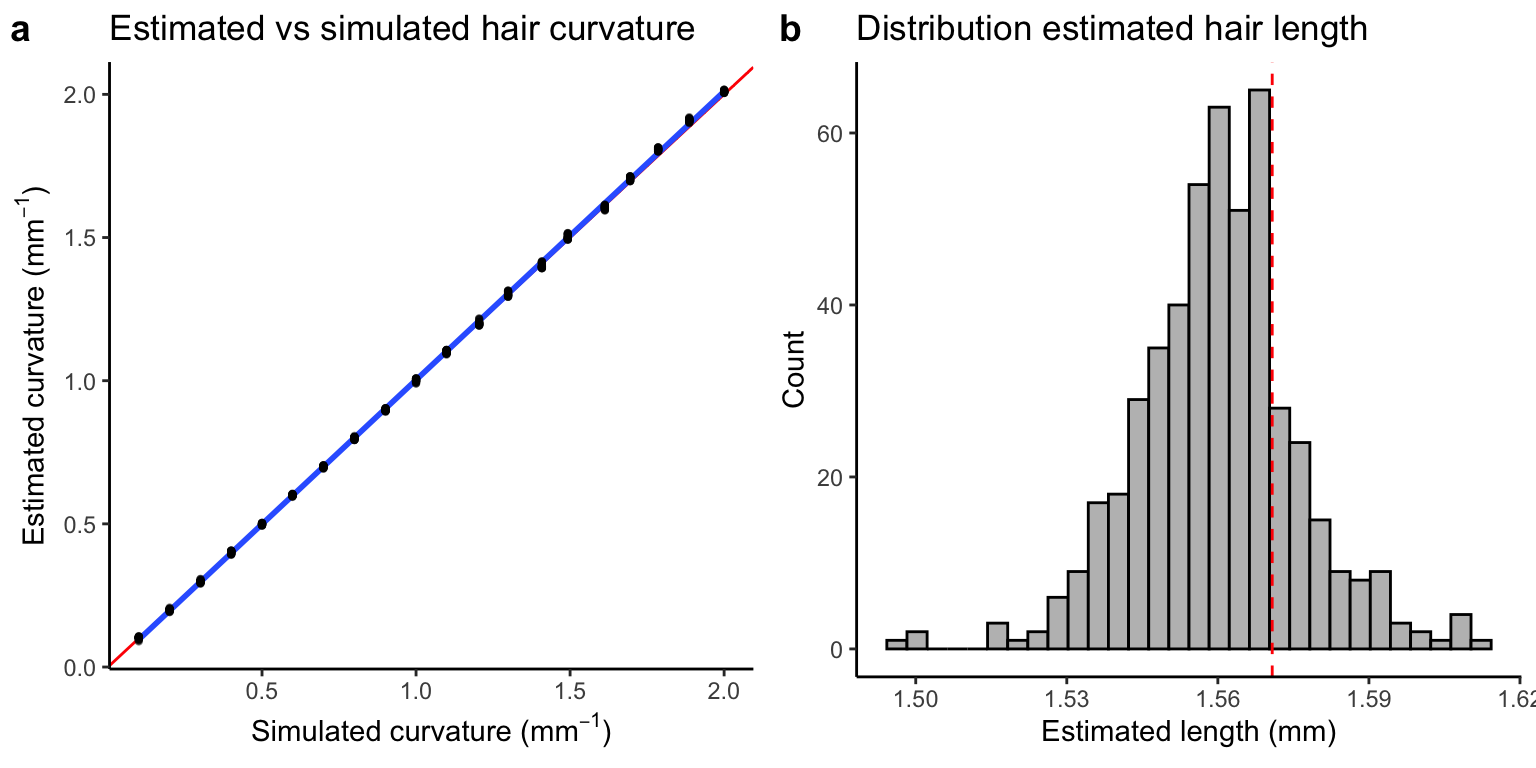
\includegraphics[width=1\linewidth]{validation_files/figure-latex/plt_curvature_corr_length-1} \caption{Error in estimated curvature and length}\label{fig:plt_curvature_corr_length}
\end{figure}

In Fig. 1a we see that there is a near perfect correlation between the
simulated and estimated curvatures. Fig. 1b shows the distribution of
estimated hair lengths around the simulated length (red line).

We plot simulated curvature against estimated length to show the
distribution of estimated length as a function of curvature.

\begin{figure}
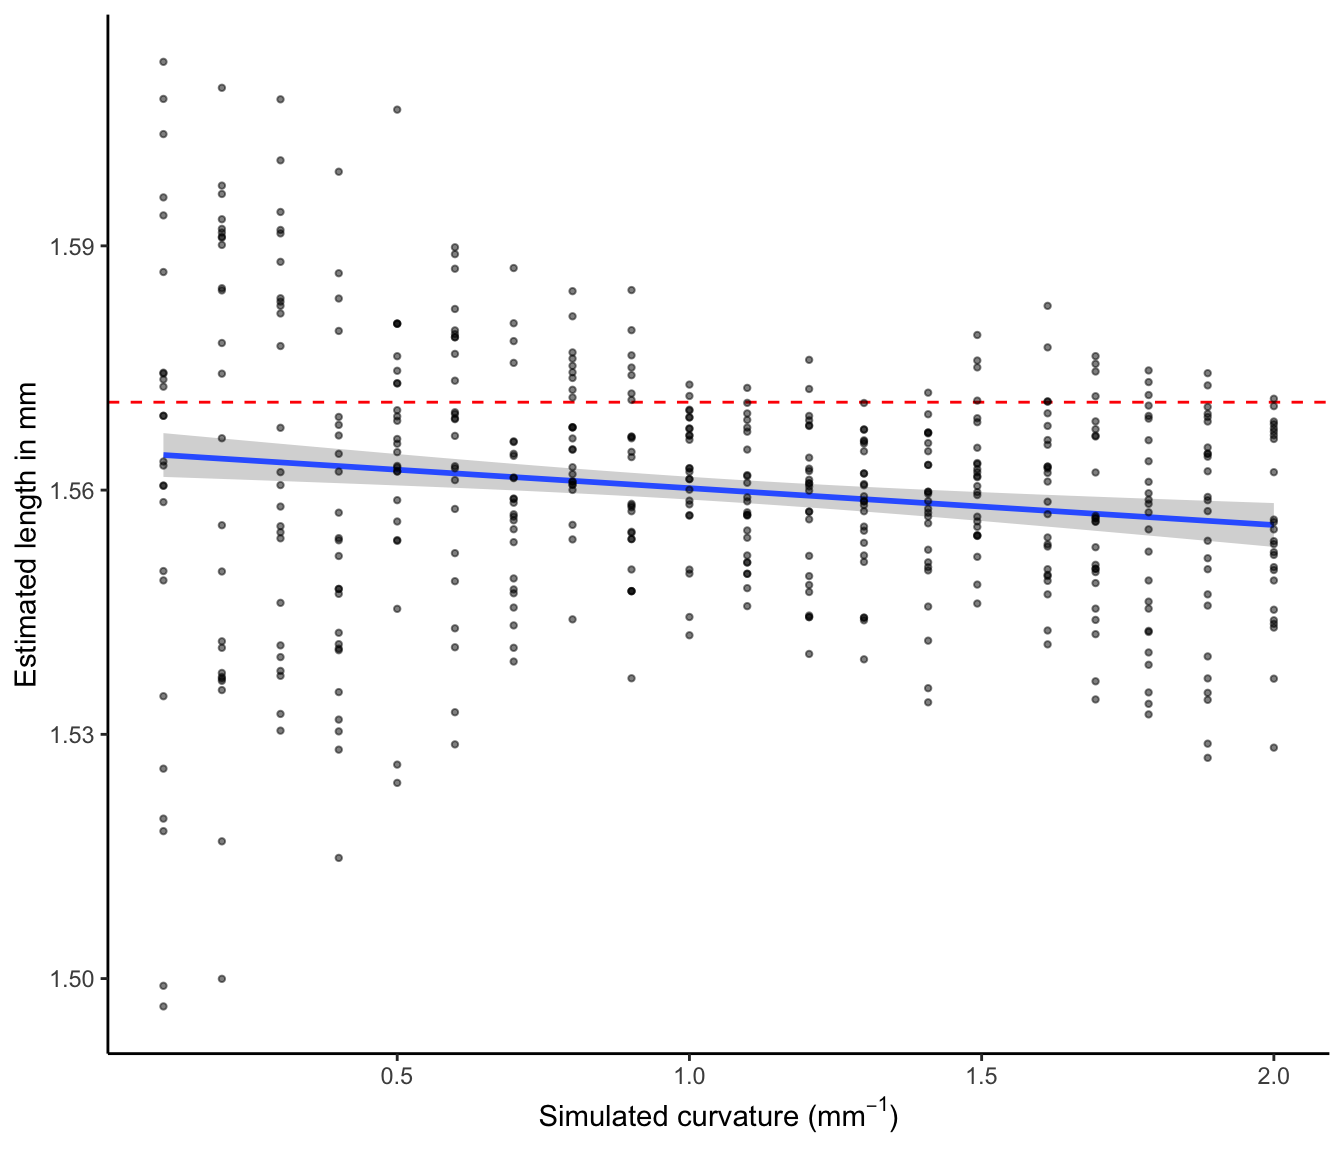
\includegraphics[width=1\linewidth]{validation_files/figure-latex/plt_length_curv-1} \caption{Simulated curvature vs estimated length}\label{fig:plt_length_curv}
\end{figure}

Figure 2 shows a broader range of error in the estimation of length in
straighter hairs. This is likely a result of the majority of pixels
being oriented in a manner that causes a divergence between the pixel
length (number of pixels) and the real length that is being measured. We
apply a correction for this known issue in image analysis, however, it
is expected that there will still be some error. Note that each point in
this figure represents an individual hair fragment within an image. This
supports the notion that it is not the low curvature per se, but rather
the combination of low curvature and specific orientations that
increases the error in length estimation.

\hypertarget{measurement-error-in-curvature-and-length}{%
\subsection{Measurement error in curvature and
length}\label{measurement-error-in-curvature-and-length}}

In addition to the correlations between simulated and estimated
parameters, we calculate root mean square error (RMSE) and percent error
as alternatives to investigate the measurement error of our package.

NB: we present the data summarized for each image (i.e.~all 25
fragments) as we cannot provide a hair fragment to hair fragment
comparison.

\hypertarget{error-statistics}{%
\subsubsection{Error statistics}\label{error-statistics}}

Below, we calculate the mean error values for both RMSE and percent
error.

\begin{longtable}[]{@{}lrr@{}}
\caption{RMSE and Percent Error per variable}\tabularnewline
\toprule
var & mean.rmse & perent.error\tabularnewline
\midrule
\endfirsthead
\toprule
var & mean.rmse & perent.error\tabularnewline
\midrule
\endhead
curvature & 0.0002210 & 0.4720430\tabularnewline
length & 0.0004312 & 0.6863358\tabularnewline
radius & 0.0004624 & 0.4626120\tabularnewline
\bottomrule
\end{longtable}

We see less than 1\% error across the variables and RMSE of less than
0.0005.

Below, we plot the data.

\hypertarget{root-mean-square-error}{%
\subsubsection{Root mean square error}\label{root-mean-square-error}}

First, we plot the root mean square error for curvature and length.

\begin{figure}
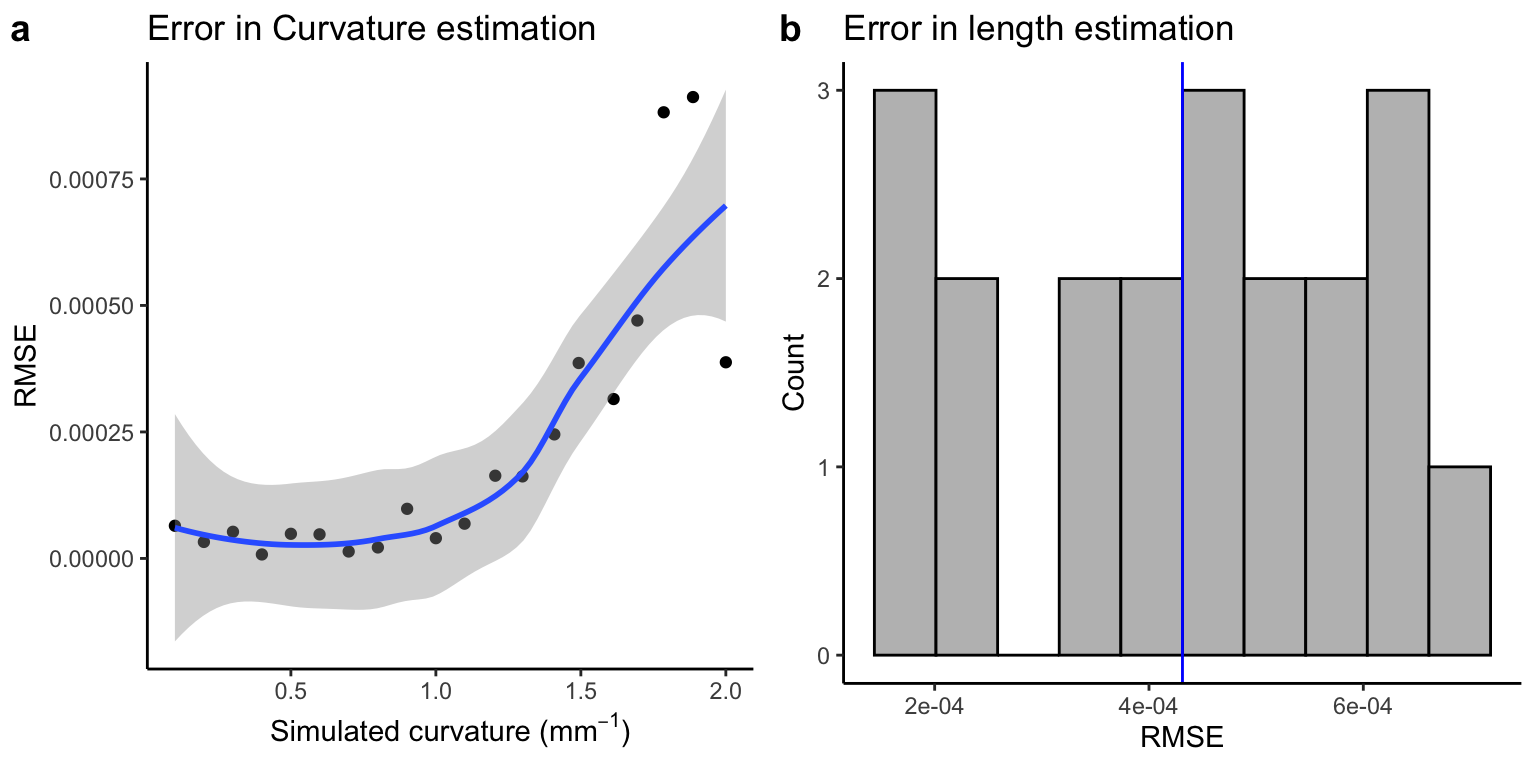
\includegraphics[width=1\linewidth]{validation_files/figure-latex/plt_rmse_curv-1} \caption{Root mean square error for curvature and length}\label{fig:plt_rmse_curv}
\end{figure}

We then examine the relationship between curvature and RMSE of length

\begin{figure}
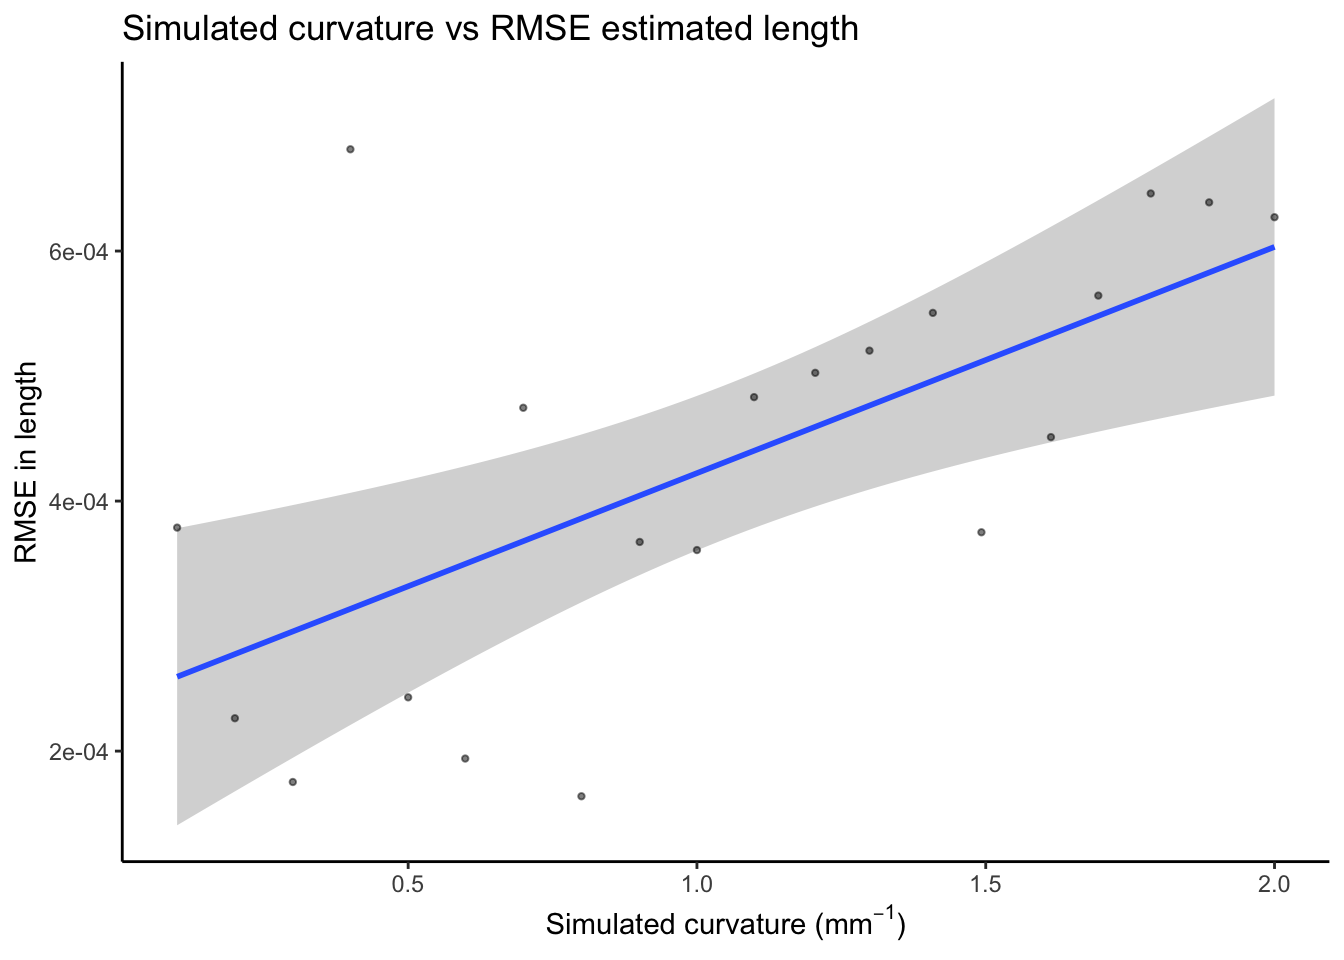
\includegraphics[width=1\linewidth]{validation_files/figure-latex/plt_length_curv_rmse-1} \caption{Correlation between curvature and RMSE for length}\label{fig:plt_length_curv_rmse}
\end{figure}

We observe an increase in RMSE with curvature.

\hypertarget{percent-error}{%
\subsubsection{Percent error}\label{percent-error}}

Below we plot the percent error for curvature and length.

\begin{figure}
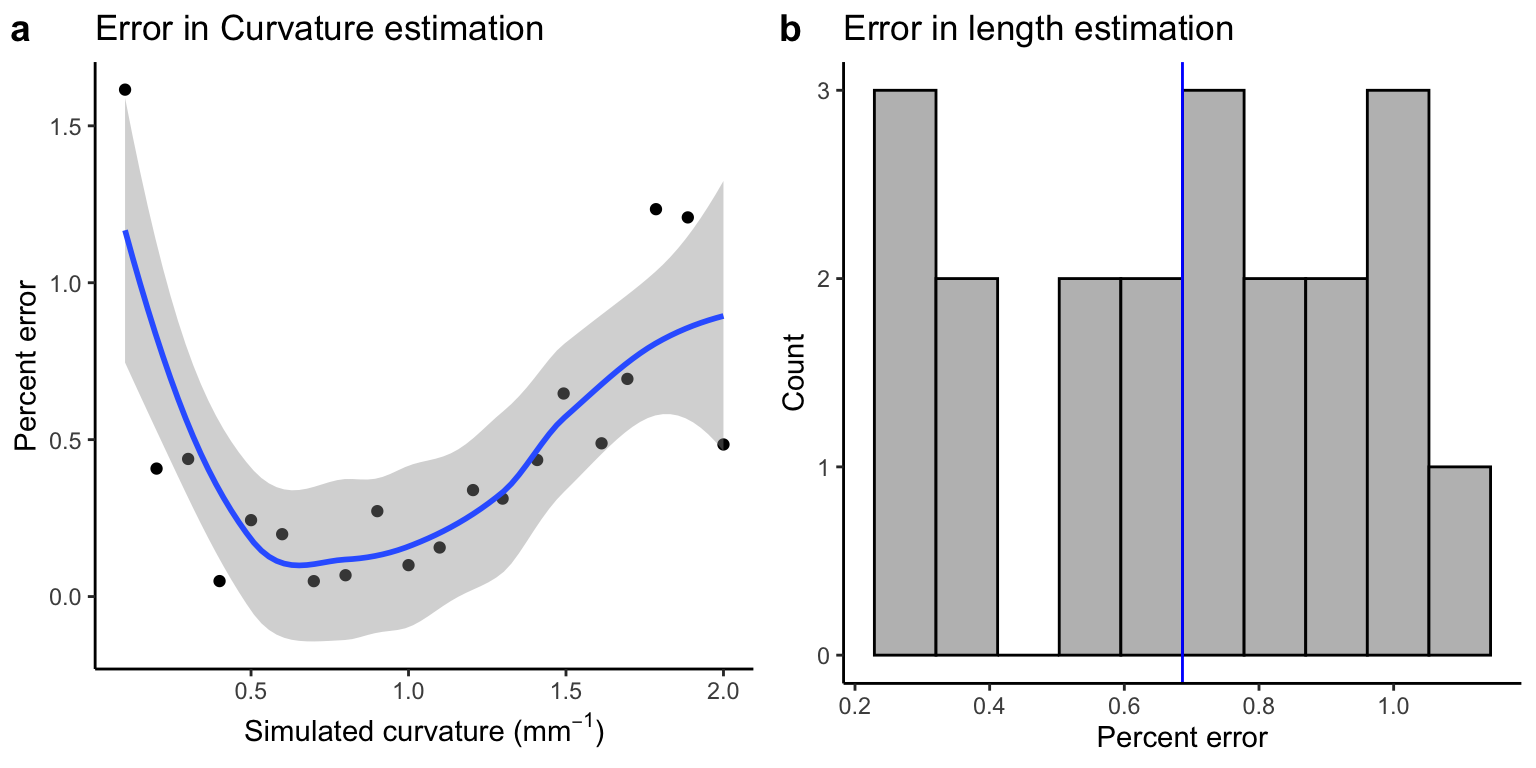
\includegraphics[width=1\linewidth]{validation_files/figure-latex/plt_perror_curv-1} \caption{Percent error for curvature and length}\label{fig:plt_perror_curv}
\end{figure}

\begin{figure}
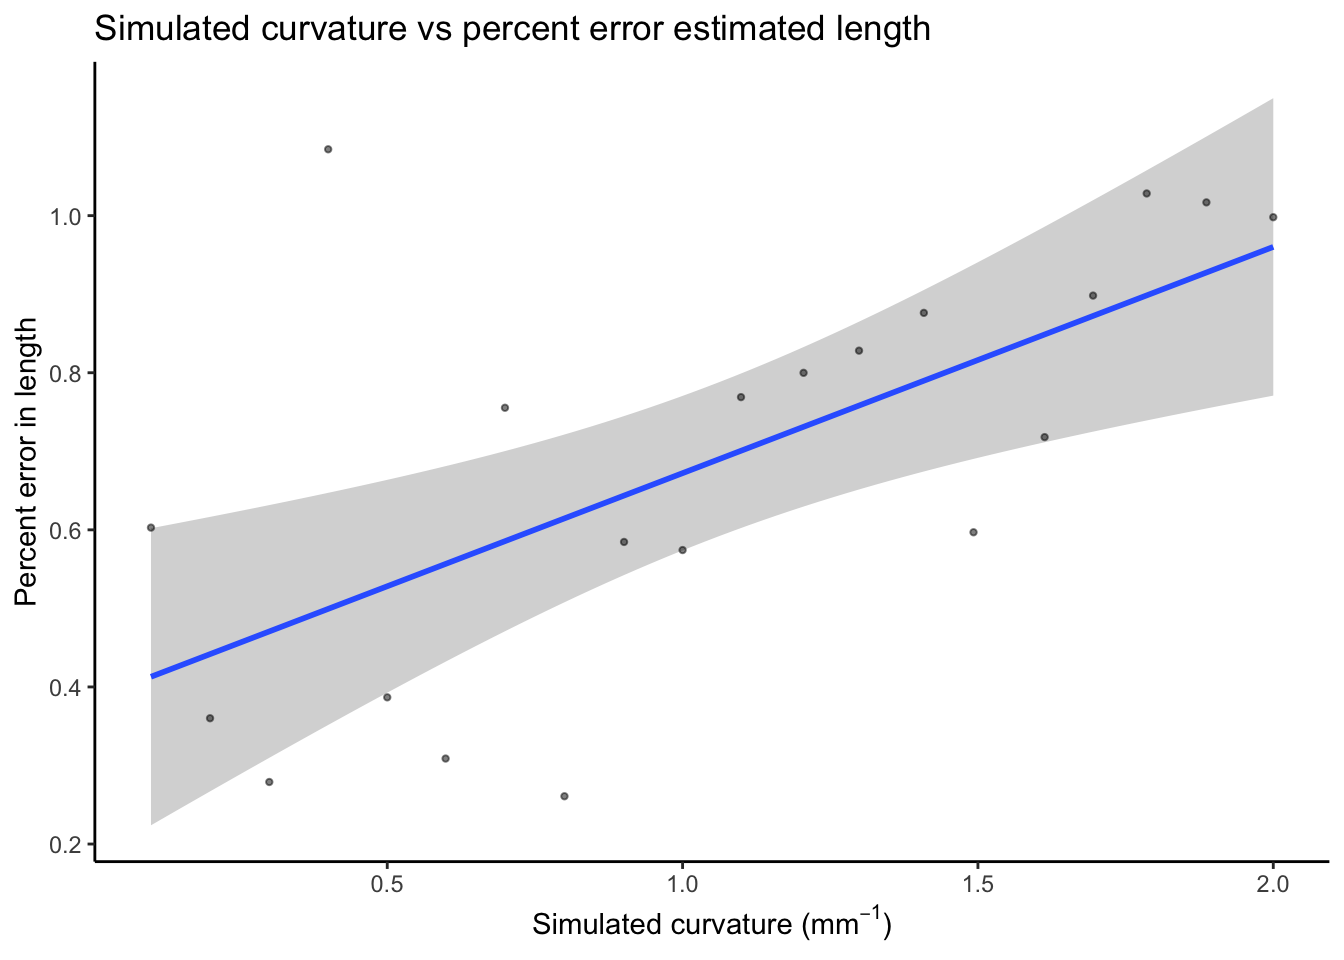
\includegraphics[width=1\linewidth]{validation_files/figure-latex/plt_length_curv_perror-1} \caption{Correlation between curvature and percent error for estimated length}\label{fig:plt_length_curv_perror}
\end{figure}

Here we see that error appears to increase slightly with curvature if
considering the data in terms of percent error.

\hypertarget{cross-section}{%
\section{Cross-section}\label{cross-section}}

The fibermorph section function estimates area, minimum diameter,
maximum diameter and eccentricity for a given cross-sectional image. We
tested the measurement error using randomly generated circles and
non-circular ellipses.

\hypertarget{correlation-between-simulated-and-estimated-section-parameters}{%
\subsection{Correlation between simulated and estimated section
parameters}\label{correlation-between-simulated-and-estimated-section-parameters}}

\begin{figure}
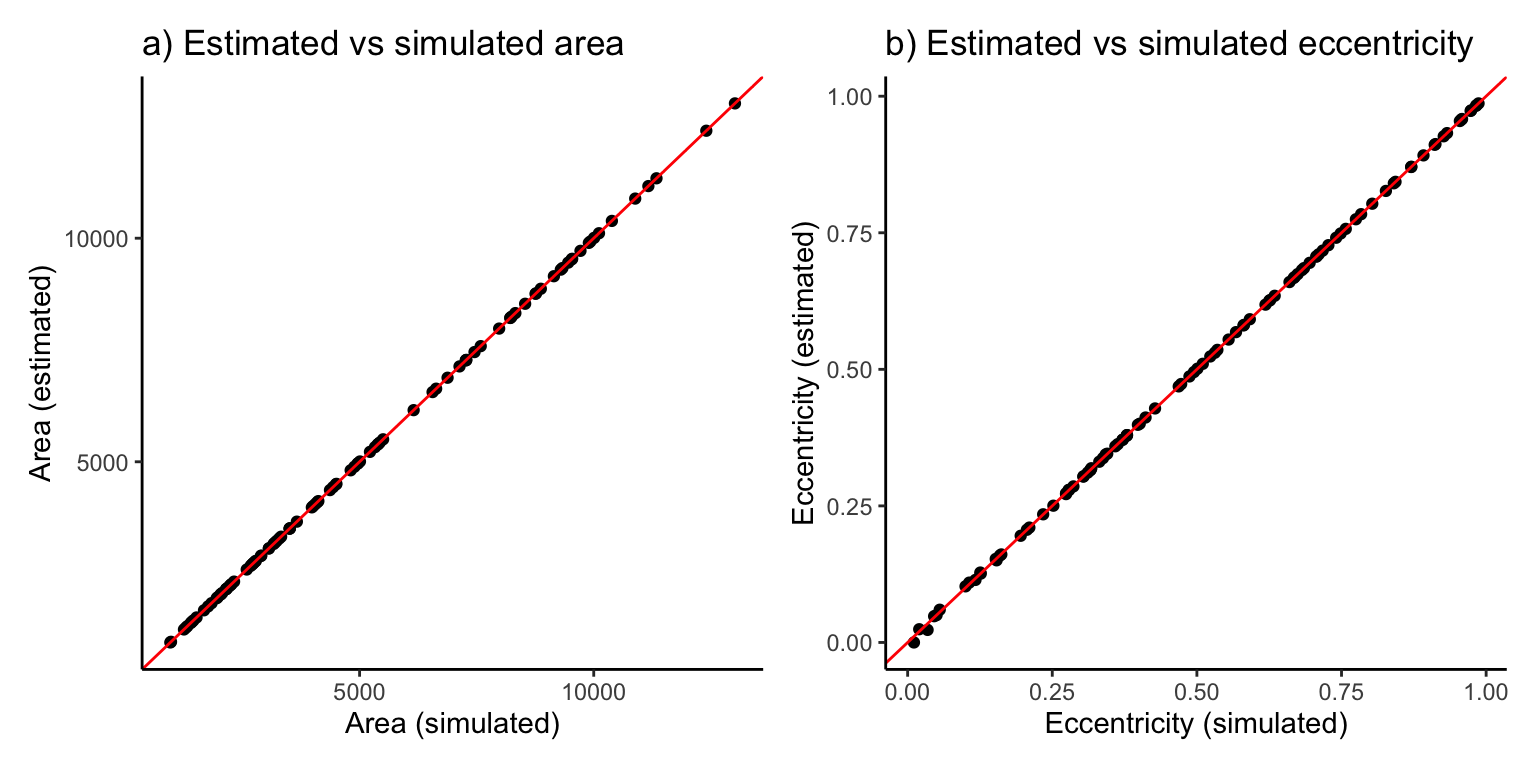
\includegraphics[width=1\linewidth]{validation_files/figure-latex/plt_section_correlation-1} \caption{FCorrelation between simulated and estimated cross-sectional parameters}\label{fig:plt_section_correlation}
\end{figure}

We see strong correlations between the estimated and simulated values
for each cross-sectional parameter.

\hypertarget{measurement-error-for-cross-sectional-parameters}{%
\subsection{Measurement error for cross-sectional
parameters}\label{measurement-error-for-cross-sectional-parameters}}

We calculate the percent error and RMSE for the cross-sectional
parameters.

First, we calculate mean error values for all parameters.

\begin{longtable}[]{@{}lrr@{}}
\caption{RMSE and Percent Error per variable}\tabularnewline
\toprule
var & mean\_rmse & perent\_error\tabularnewline
\midrule
\endfirsthead
\toprule
var & mean\_rmse & perent\_error\tabularnewline
\midrule
\endhead
area & 0.5136320 & 0.0137703\tabularnewline
eccentricity & 0.0007514 & Inf\tabularnewline
max & 0.0097800 & 0.0120605\tabularnewline
min & 0.0080884 & 0.0136924\tabularnewline
\bottomrule
\end{longtable}

Percent error is considerably under 0.02\% for each of the parameters
with RMSE under 0.01 for all but area.

As one of the simulated ellipses was a circle with an eccentricity of 0,
any deviation from this produces an infinite percent error. So below we
present the values removing this observation.

\begin{longtable}[]{@{}lrr@{}}
\caption{RMSE and Percent Error per variable}\tabularnewline
\toprule
var & mean\_rmse & perent\_error\tabularnewline
\midrule
\endfirsthead
\toprule
var & mean\_rmse & perent\_error\tabularnewline
\midrule
\endhead
area & 0.5136320 & 0.0137703\tabularnewline
eccentricity & 0.0006492 & 1.0066337\tabularnewline
max & 0.0097800 & 0.0120605\tabularnewline
min & 0.0080884 & 0.0136924\tabularnewline
\bottomrule
\end{longtable}

\hypertarget{root-mean-square-error-1}{%
\subsubsection{Root mean square error}\label{root-mean-square-error-1}}

Below, we plot RMSE as a function of each parameter.

\begin{figure}
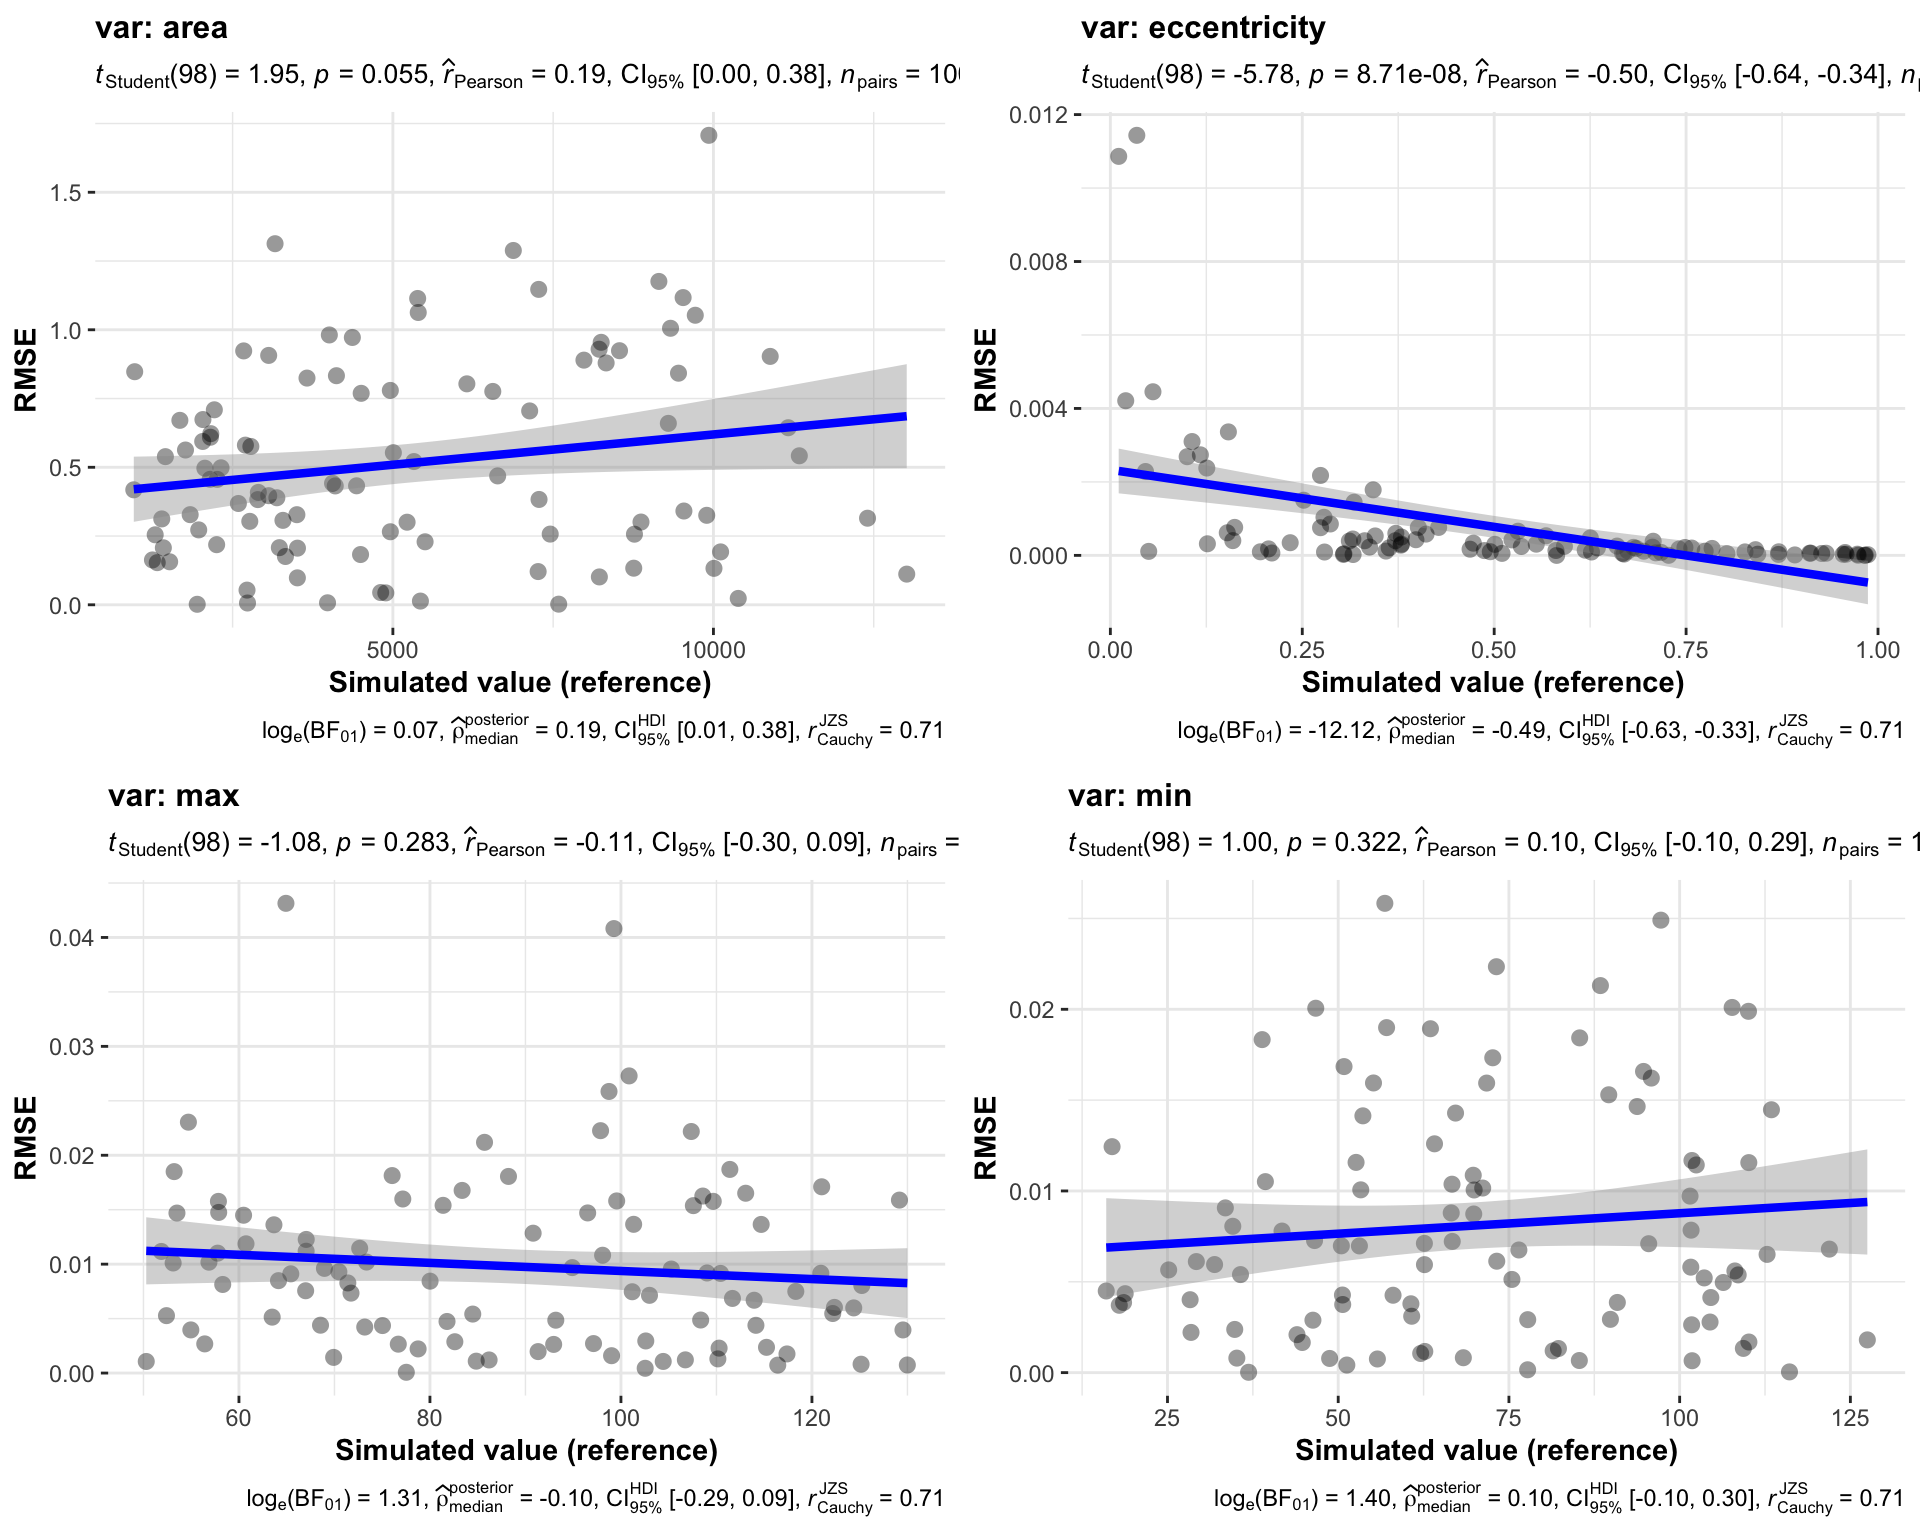
\includegraphics[width=1\linewidth]{validation_files/figure-latex/plt_section_RMSE-1} \caption{Correlation between simulated and RMSE for cross-sectional parameters}\label{fig:plt_section_RMSE}
\end{figure}

There does not appear to be any overarching pattern in RMSE across the
variables.

\hypertarget{percent-error-1}{%
\subsubsection{Percent error}\label{percent-error-1}}

Below we plot the correlation between simulated values and percent error
for each parameter.

\begin{figure}
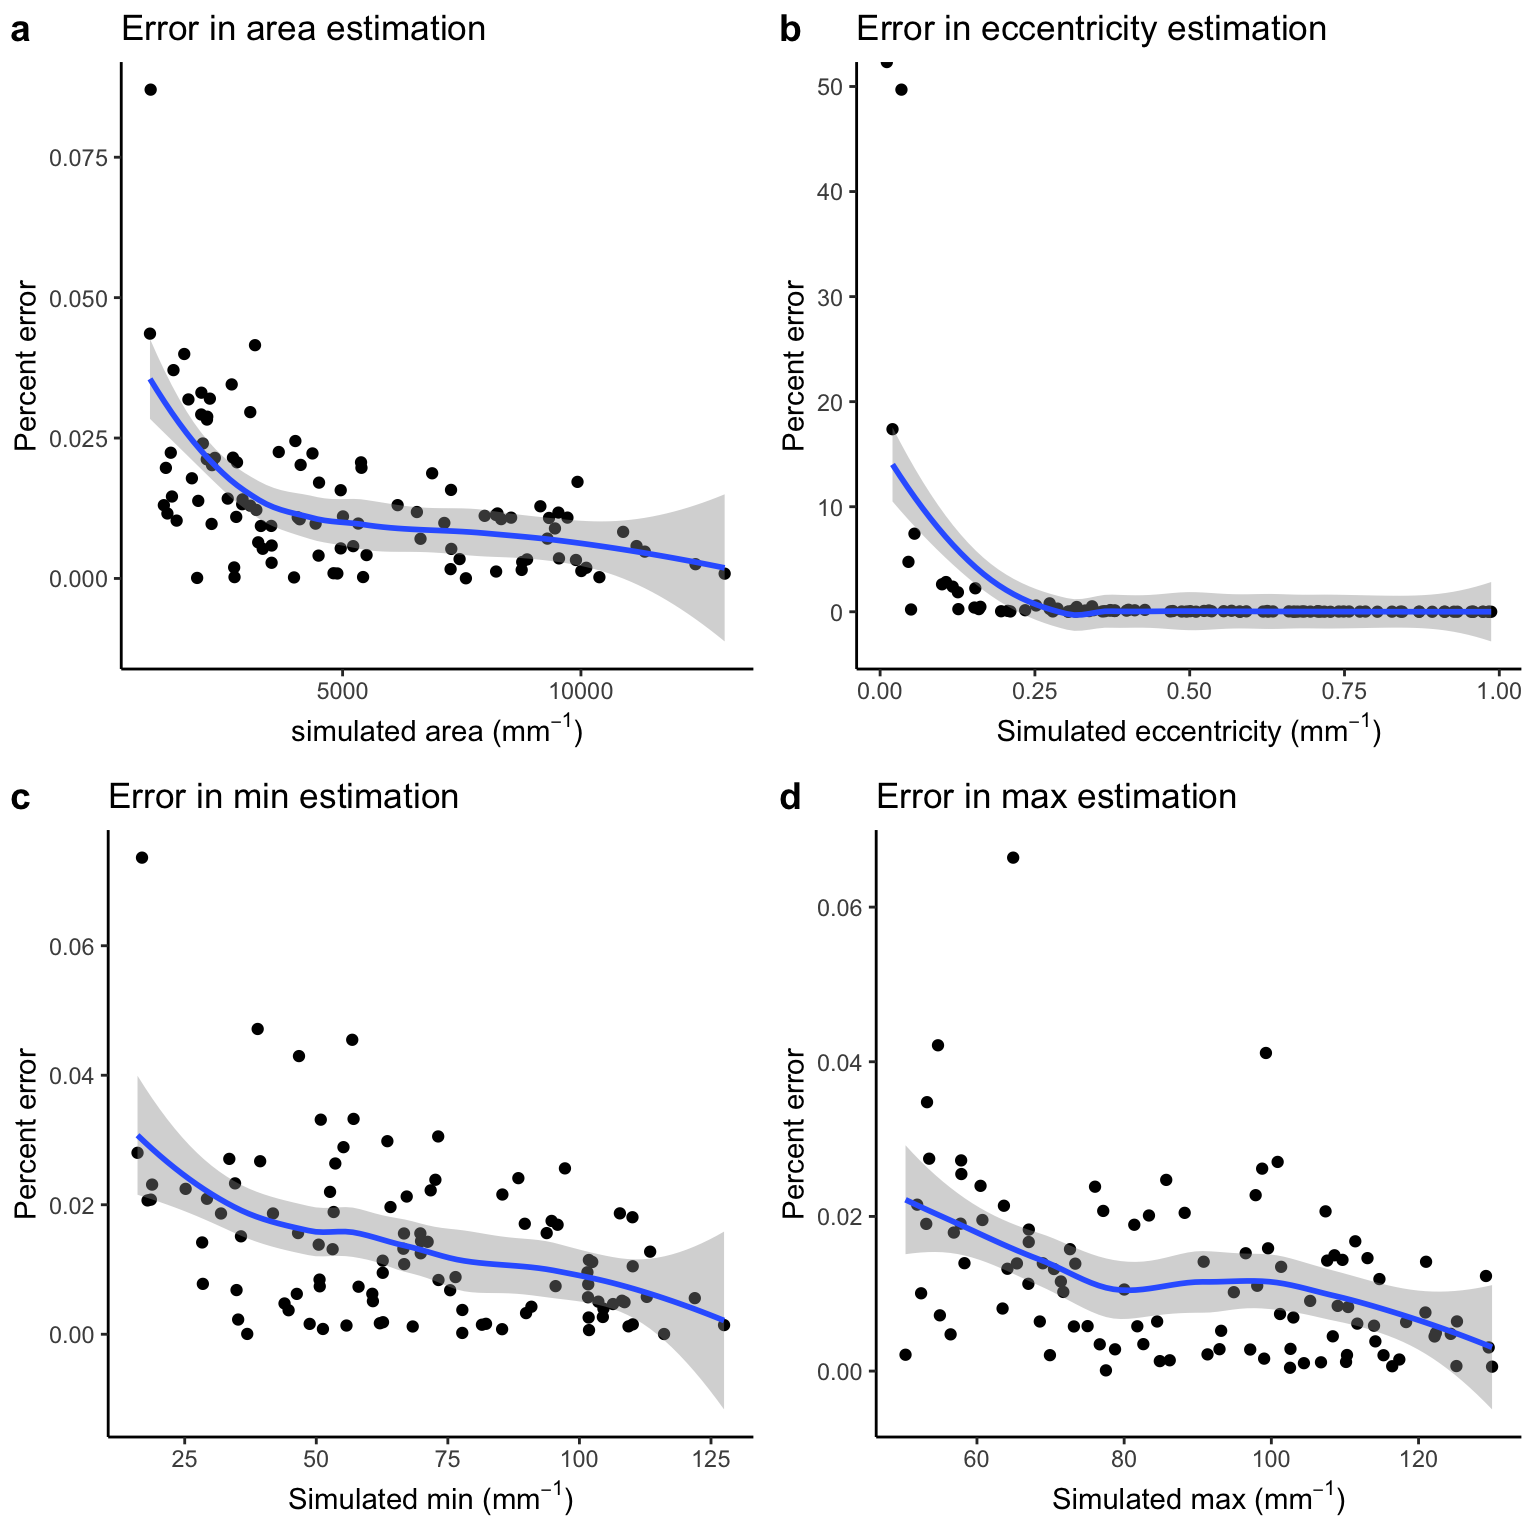
\includegraphics[width=1\linewidth]{validation_files/figure-latex/plt_section_corr-1} \caption{Correlation between simulated and percent error cross-sectional parameters}\label{fig:plt_section_corr}
\end{figure}

We observe a general decrease in percent error for each parameter.

\end{document}
